\documentclass[11pt,a4paper]{article}
\usepackage[margin=1in]{geometry}
\usepackage{booktabs}
\usepackage{graphicx}
\usepackage{amsmath}
\usepackage{caption}
\usepackage[hidelinks]{hyperref}
\usepackage{setspace}
\setstretch{1.04}
\captionsetup{font=small,labelfont=bf}
\newif\ifanon
\ifx\anon\undefined\anonfalse\else\anontrue\fi

\title{What the Record Remembers: Snapshot Leakage in Predicting Exploited Vulnerabilities from Public CVE Data}
\ifanon
\author{Anonymous Submission}
\else
\author{Hilux Fokou Ngoumo\\ \small Information Security Programme, ITMO University, Saint Petersburg, Russia}
\fi
\date{}

\begin{document}
\maketitle

\begin{abstract}
Machine learning models that predict which software vulnerabilities will be exploited are usually trained on public CVE records and labeled with the CISA Known Exploited Vulnerabilities (KEV) catalog. These records are living documents. They are edited, enriched and cross-referenced long after publication, and some of the edits are made precisely because a vulnerability was exploited. A model trained on today's copy of a record can therefore see information that did not exist when the vulnerability was disclosed. I study this problem on 183,409 CVEs published between November 2021 and July 2026, with a 90-day exploitation label taken from KEV (587 positives). I split the available record fields into a disclosure-time safe set and five groups that are contaminated by later events, and I evaluate a logistic regression model on each combination under random cross-validation and under forward-in-time splits. Two fields written by CISA's own enrichment container turn the task into a lookup: with them average precision rises from about 0.08 to about 0.85 on future CVEs, and the KEV flag is literally present in every positive record. Fields that look harmless, such as references, CVSS temporal metrics and the lag between publication and last update, lift random-split scores without being exact label copies. Random cross-validation on safe features alone already overstates average precision by roughly a factor of three compared with forward-in-time testing (0.23 against 0.08). Making the training labels aware of the label delay changed little at 30 and 90 days, because most KEV entries arrive within weeks of publication, but it mattered at 365 days. On a clean forward-in-time test, a simple model using only CNA-supplied fields reaches an AUROC of 0.86 to 0.93 and ranks far better than CVSS severity (0.64 to 0.67), but its precision is low, and I report that openly. I close with an audit checklist for work that predicts exploitation from CVE records, and I release the code and the derived feature tables.
\end{abstract}

\noindent\textbf{Keywords:} vulnerability exploitation prediction, CISA Known Exploited Vulnerabilities, CVE, data leakage, temporal evaluation, machine learning for security, vulnerability prioritization

\section{Introduction}

Organizations learn about tens of thousands of new vulnerabilities each year, and only a small fraction is ever used in an attack. Choosing which ones to fix first is a prediction problem, and a growing body of work tries to solve it with statistical models trained on public data \cite{bozorgi2010,sabottke2015,jacobs2019,suciu2022,jacobs2023}. The most convenient source of ground truth today is the Known Exploited Vulnerabilities (KEV) catalog that the US Cybersecurity and Infrastructure Security Agency (CISA) has maintained since November 2021 under Binding Operational Directive 22-01 \cite{bod2201,kev}. The most convenient source of features is the CVE List itself, where each record carries a description, weakness types, affected products, references and scores.

The difficulty is that a CVE record is not a fixed object. It is a document that keeps changing. A vendor adds an advisory link, a researcher adds a proof-of-concept reference, a scoring body adds a severity vector, and an enrichment program adds a machine-readable note about exploitation status. When a model is trained on the current version of every record, the features describe the world as it is today, while the question being asked is about the world on the day of disclosure. I call the resulting problem \emph{snapshot leakage}. It is related to the temporal bias that Pendlebury et al.\ documented for malware classifiers \cite{pendlebury2019} and to the leakage taxonomy of Kapoor and Narayanan \cite{kapoor2023}, but it has a particular shape here: the leak enters through the text and metadata of a public record, and some of it is put there by the same agency that produces the labels.

Prior work has noticed parts of the problem. Yang et al.\ argued that reference links should not be used as features because links to proof-of-concept code carry the answer \cite{yang2020}. Iannone et al.\ built time-aware evaluations for just-disclosed vulnerabilities and showed that realistic performance is modest \cite{iannone2024}. A recent preprint proposes a leakage-safe triage protocol that admits only evidence visible by a decision time \cite{alpay2026}. What I could not find is a measurement of how much each family of record fields contributes to inflated performance when the labels come from KEV, how that compares with the inflation from evaluation design alone, and whether the label delay (a CVE published last month cannot yet have been listed) matters in practice.

I address four questions on one fully public dataset.
\begin{itemize}
\item \textbf{RQ1.} Which groups of CVE record fields carry information that was not available at disclosure, and how much does each inflate performance?
\item \textbf{RQ2.} How much does random cross-validation overstate performance compared with forward-in-time testing when only safe fields are used?
\item \textbf{RQ3.} Does a label-delay-aware training cutoff change the results compared with training on every earlier CVE using today's labels?
\item \textbf{RQ4.} What can a model using only disclosure-time fields actually do, compared with severity-score and vendor-history baselines?
\end{itemize}

My contributions are the following. First, an explicit partition of CVE record fields into a safe set and five contaminated groups, with the evidence for each assignment. Second, a controlled comparison of these groups under random and forward-in-time evaluation on 183,409 CVEs. Third, an honest estimate of what a transparent model can achieve on safe fields alone. Fourth, a short audit checklist and a public release of the pipeline.

\section{Background and Related Work}

\paragraph{Exploit prediction.} Bozorgi et al.\ were among the first to learn exploitation from vulnerability metadata \cite{bozorgi2010}. Sabottke et al.\ added social media signals \cite{sabottke2015}. The Exploit Prediction Scoring System (EPSS) combines many features and publishes daily probabilities, and its later versions use data from community sources and observed exploitation activity \cite{jacobs2019,jacobs2023}. Suciu et al.\ predict whether a functional exploit will be developed \cite{suciu2022}. Allodi and Massacci showed with case-control studies that CVSS severity is a weak guide to attacks in the wild \cite{allodi2014}, and Spring et al.\ discussed how CVSS would need to change to serve prioritization better \cite{spring2021}. The Stakeholder-Specific Vulnerability Categorization (SSVC) from the CERT Coordination Center takes a decision-tree approach and includes an exploitation status input \cite{ssvc}.

\paragraph{Data quality and leakage.} Anwar et al.\ assessed the quality of National Vulnerability Database records and found inconsistencies in their fields \cite{anwar2022}. In machine learning for security more generally, Arp et al.\ list temporal snooping and sampling bias among common pitfalls \cite{arp2022}. Kapoor and Narayanan survey leakage across scientific fields \cite{kapoor2023}, and Geirhos et al.\ describe how models latch onto shortcuts that happen to correlate with labels \cite{geirhos2020}. In the exploit-prediction setting, Yang et al.\ found that reference hosts that serve proof-of-concept code help models in a way that should not be trusted \cite{yang2020}, using Exploit-DB labels and cvedetails data. Iannone et al.\ evaluate prediction from the early content of a CVE in a time-aware setup and report performance that falls in recent years \cite{iannone2024}. Alpay and Alpay propose evidence certificates and a decision-time cutoff for each CVE, using retrieval over discussion corpora, and show that naive protocols inflate recall \cite{alpay2026}.

\paragraph{What is different here.} The above work either argues for one source of leakage, or builds a larger system with a leakage-safe protocol. I instead hold the model fixed and simple, and vary only which record fields it may see and how it is evaluated. This isolates the contribution of each field group. Because the data are the CVE List, the CISA enrichment repository and KEV, all of which are public and versioned on GitHub, the experiments can be repeated by anyone.

\section{Data}

\paragraph{Sources.} I cloned three public repositories: the CVE List in the CVE JSON 5 format (cvelistV5), the CISA Vulnrichment repository that stores the enrichment container CISA adds to CVE records, and the KEV catalog data. The KEV file used here is catalog version 2026.10.08 with 1{,}739 entries. All 404{,}031 CVE JSON files were parsed into a flat table. I kept records in the published state (385{,}568) and recorded, for each, the fields supplied by the CVE Numbering Authority (CNA), the fields added by later containers, the dates, and the KEV addition date when present.

\paragraph{Cohort.} The KEV catalog started on 3 November 2021, so I only keep CVEs published from that date. Because a label with horizon $H$ days is only observable when $H$ days have passed since publication, the cohort for horizon $H$ ends $H$ days before the KEV snapshot. For the main horizon $H=90$ this gives 183{,}409 CVEs published between 3 November 2021 and 10 July 2026. A CVE is positive if its KEV addition date is at most $H$ days after its publication date. There are 587 positives (0.32\%). KEV also contains CVEs that were added the same day they were published, or before, and I count those as positive with a time to KEV of zero or less. Of the 790 KEV entries inside the cohort window, 25.6\% were added on or before the publication date, 47.7\% within a week, 61.1\% within 30 days, 74.3\% within 90 days and 91.6\% within a year; the median is 9 days (Figure~\ref{fig:ttk}). The year-by-year positive counts at $H=90$ are 10 (2021, partial), 85, 121, 113, 159 and 99 for 2026.

\begin{figure}[t]
\centering
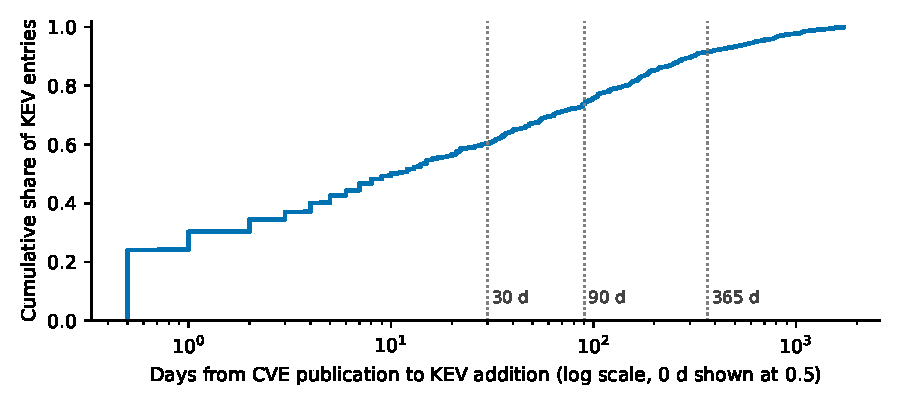
\includegraphics[width=0.78\linewidth]{figs/fig_ttk.pdf}
\caption{Time from CVE publication to KEV addition for KEV entries in the cohort. Most additions come within weeks, which is why the label delay turns out to matter little for the 90-day horizon.}
\label{fig:ttk}
\end{figure}

\paragraph{Feature groups.} The central design choice is the split of fields into groups, summarized in Table~\ref{tab:groups}. The safe set $S$ contains fields that a CNA supplies when it publishes the record: the CNA's base CVSS v3 and v4 vector components and score, weakness (CWE) identifiers, affected vendors and products, whether product identifiers (CPE) are present, the assigning CNA, the length and word content of the title and description, and the time between ID reservation and publication. It is not perfectly clean, because a CNA can also edit its own record later, and I return to this in Section~\ref{sec:limits}. Each contaminated group is one whose content is known to be able to change after publication in response to exploitation or attention:
\begin{itemize}
\item \textbf{C\_temporal}: the CVSS temporal metrics (exploit code maturity, remediation level, report confidence) in the CNA vector, and the v4 exploit maturity.
\item \textbf{C\_refs}: reference domains, reference tags and the number of references.
\item \textbf{C\_update}: the number of days between the published and last-updated timestamps.
\item \textbf{C\_enrich}: the number and names of enrichment (ADP) containers, the SSVC decision options and the ADP references.
\item \textbf{C\_kevfield}: the \texttt{kev} block that the CISA enrichment container adds to a record and the KEV reference link.
\end{itemize}

\begin{table}[t]
\centering
\caption{Prevalence of leakage indicators in the 90-day cohort, in positives (587) and negatives (182{,}822). The negatives include 203 CVEs that entered KEV later than 90 days, which explains the small nonzero shares in the first rows.}
\label{tab:groups}
\small
\begin{tabular}{llrr}
\toprule
Group & Indicator & Positives & Negatives \\
\midrule
C\_kevfield & CISA \texttt{kev} block in the record & 100\% & 0.11\% \\
C\_enrich & SSVC exploitation value ``active'' & 100\% & 0.11\% \\
C\_enrich & SSVC container present & 100\% & 84.1\% \\
C\_temporal & CVSS exploit maturity ``F'' or ``H'' & 14.0\% & 0.21\% \\
Text (set S) & ``in the wild'' in the description & 11.1\% & 0.09\% \\
C\_update & Updated more than 30 days after publication & 95.7\% & 66.8\% \\
C\_update & Median days between publication and last update & 501 & 241 \\
C\_refs & Reference tagged vendor advisory & 35.6\% & 12.9\% \\
C\_refs & Reference to a GitHub repository & 9.2\% & 30.0\% \\
C\_refs & Reference to packetstormsecurity.com & 8.3\% & 0.74\% \\
\bottomrule
\end{tabular}
\end{table}

The first rows of Table~\ref{tab:groups} show the problem in its plainest form. Every positive CVE carries the CISA \texttt{kev} block, because the block is how the enrichment program records KEV membership. A model that sees this field is not predicting anything. The SSVC ``active'' exploitation value behaves the same way. The pattern in the reference rows is different and more interesting: positives are \emph{less} likely to cite GitHub than negatives and more likely to cite vendor advisories and Packet Storm. These are statistical shadows of exploitation, not copies of the label, and they are the kind of feature that a careful-looking study could include without noticing a problem.

\section{Method}

\paragraph{Models and features.} For every configuration I fit an L2-regularized logistic regression (liblinear solver, $C=1$) on a sparse matrix built from the training portion only: standardized numeric features, one-hot encodings of the CVSS components and the assigning CNA, binary indicators for CWE, vendor and product tokens, and TF-IDF features (unigrams and bigrams, at most 30{,}000) of the title and description. I chose a linear model on purpose. It is transparent, fast, and it makes differences between feature groups easy to attribute. The first column of Table~\ref{tab:main} labels each configuration: $S$ alone, $S$ plus one contaminated group, and $S$ plus all of them.

\paragraph{Protocols.} \emph{Random} evaluation uses stratified 5-fold cross-validation with a fixed shuffle seed. \emph{Temporal} evaluation tests on all CVEs published in one calendar year (2024, 2025 or 2026) and trains only on earlier ones, in two ways. The \emph{naive} variant trains on every CVE published before the test year, labeled with the final snapshot. The \emph{delay-aware} variant trains only on CVEs published at least $H$ days before the start of the test year, so that every training label has had its full observation window before the model would have been deployed. The 2026 test year runs through the end of the cohort in July.

\paragraph{Metrics.} The positive class is rare, so I report average precision (AP) as the main metric, together with AUROC, precision in the top 1\% of the ranking and recall in the top 5\%. For single test years I give 95\% bootstrap intervals from 200 resamples of the test set. I also report three rule baselines: ranking by CVSS base score, ranking by the easiest network attack vector (AV:N, AC:L, PR:N, UI:N) with score as tie-break, and a vendor prior (the training positive rate of the vendor string, smoothed toward the global rate).

\paragraph{Ablations.} To see whether text features rely on wording that gives exploitation away, I remove sentences containing words like ``exploited'', ``in the wild'', ``actively'', ``proof of concept'' and ``attack'' from titles and descriptions and refit the safe model. I also fit the safe model without any text features. Finally I repeat the main experiment with horizons of 30 and 365 days.

\section{Results}

\subsection{Contaminated fields inflate performance (RQ1)}

Table~\ref{tab:main} and Figure~\ref{fig:ap} give the main comparison at $H=90$. Under every protocol, the two enrichment-related groups (C\_enrich and C\_kevfield) turn the task into a near-lookup: AUROC is 0.999 or higher and AP is about 0.82 to 0.87 on future CVEs, against 0.07 to 0.08 for the safe set. Adding the CVSS temporal metrics roughly doubles temporal AP to 0.17 even though only 23\% of positives carry any temporal value. References and the update lag give smaller but visible increases in random AP (0.23 to 0.27 and 0.29) and in temporal AUROC for 2026 (0.88 to 0.90 and 0.92). These groups would pass a casual review, which makes them the more dangerous kind of leak.

\begin{table}[t]
\centering
\caption{Main results at $H=90$. Random: mean over 5 folds. Temporal: mean over the test years 2024, 2025 and 2026. AUROC and average precision (AP).}
\label{tab:main}
\small
\begin{tabular}{lcccccc}
\toprule
 & \multicolumn{2}{c}{Random CV} & \multicolumn{2}{c}{Temporal, delay-aware} & \multicolumn{2}{c}{Temporal, naive}\\
\cmidrule(lr){2-3}\cmidrule(lr){4-5}\cmidrule(lr){6-7}
Features & AUROC & AP & AUROC & AP & AUROC & AP \\
\midrule
Safe set S & 0.946 & 0.227 & 0.889 & 0.075 & 0.899 & 0.082 \\
S + CVSS temporal & 0.948 & 0.341 & 0.895 & 0.169 & 0.904 & 0.174 \\
S + references & 0.955 & 0.269 & 0.901 & 0.084 & 0.907 & 0.096 \\
S + update lag & 0.958 & 0.295 & 0.906 & 0.100 & 0.920 & 0.105 \\
S + ADP enrichment & 1.000 & 0.873 & 1.000 & 0.822 & 1.000 & 0.829 \\
S + KEV field & 1.000 & 0.867 & 1.000 & 0.848 & 1.000 & 0.856 \\
S + all contaminated & 1.000 & 0.889 & 1.000 & 0.869 & 1.000 & 0.872
\\
\bottomrule
\end{tabular}
\end{table}

\begin{figure}[t]
\centering
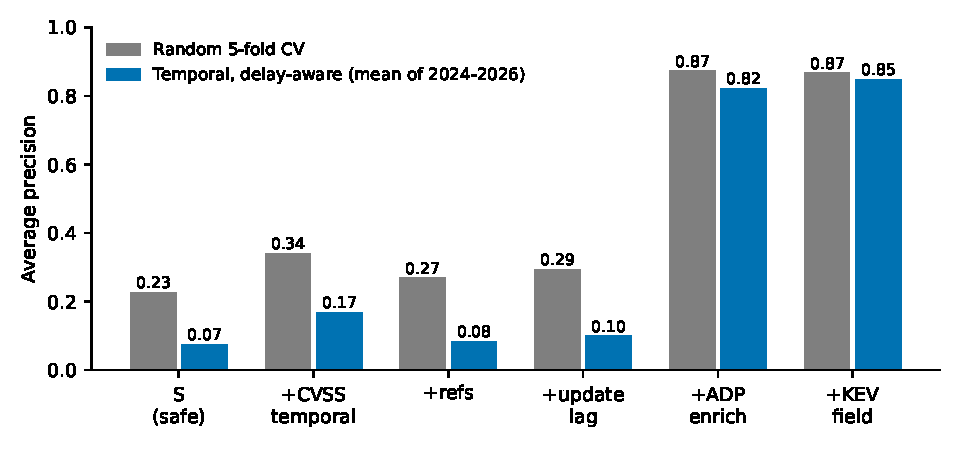
\includegraphics[width=0.85\linewidth]{figs/fig_ap.pdf}
\caption{Average precision by feature set under random cross-validation and under delay-aware temporal testing at $H=90$. The base rate of the positive class is about 0.3\%.}
\label{fig:ap}
\end{figure}

\subsection{Random cross-validation overstates performance (RQ2)}

With safe features only, random cross-validation gives an AUROC of 0.946 and an AP of 0.227. On forward-in-time test years the same model reaches an AUROC of 0.86 to 0.93 and an AP of 0.044 to 0.099 (mean 0.075). The base rate is nearly the same in both settings (0.32\% overall; 0.28\%, 0.33\% and 0.26\% in the three test years), so the gap is not a prevalence effect. Random folds put CVEs from the same vendor batches, with the same templated descriptions and the same exploited product families, on both sides of the split. A plausible reason is that the model then partly memorizes products that were popular in KEV during one period, though I did not test this directly. AP drops by about a factor of three when this memory is not allowed to help. The same pattern appears at the 30-day and 365-day horizons (Table~\ref{tab:h}).

\subsection{Label delay: small at short horizons, large at 365 days (RQ3)}

The delay-aware cutoff removes the most recent $H$ days of training data, whose labels may still change. At $H=30$ and $H=90$ it makes little difference. Delay-aware AP is 0.076 and 0.075, and naive AP is 0.086 and 0.082 (Table~\ref{tab:main}, Table~\ref{tab:h}), a gap that is small next to the year-to-year spread. The reason is visible in Figure~\ref{fig:ttk}: three quarters of KEV additions come within 90 days, and a quarter come on or before the publication date, so few positives are hidden in the final weeks before a cutoff.

At $H=365$ the picture changes. Delay-aware AP of the safe model falls to 0.032 (0.015 for 2024 and 0.049 for 2025), while naive training gives 0.072 (0.055 and 0.090). Two things differ between the variants and these runs cannot separate them. First, the naive set contains CVEs from the final year before the test period, labeled with KEV additions that happened after the test period had begun, so it uses information from the future. Second, the delay-aware set has much less data: for the 2024 test year it holds 128 positives, against 273 for naive training. The delay-aware number is the one a real deployment could have achieved, and the lesson is that a long horizon makes the choice matter, while for short horizons on KEV the delay-aware design costs very little. I would not generalize this to other label sources.

\begin{table}[t]
\centering
\caption{Sensitivity to the label horizon $H$ (days). AP of the safe model under three protocols (temporal values are means over the available test years; the 365-day cohort ends in October 2025, so it has only the test years 2024 and 2025, the second one partial), then the contaminated additions under delay-aware temporal testing.}
\label{tab:h}
\small
\begin{tabular}{rrrcccccc}
\toprule
$H$ & Cohort & Pos. & \multicolumn{3}{c}{Safe set $S$} & $S$+temporal & $S$+KEV field\\
\cmidrule(lr){4-6}
 & & & Random & Aware & Naive & Aware & Aware \\
\midrule
30 & 206,857 & 526 & 0.246 & 0.076 & 0.086 & 0.198 & 0.811 \\
90 & 183,409 & 587 & 0.227 & 0.075 & 0.082 & 0.169 & 0.848 \\
365 & 133,628 & 571 & 0.238 & 0.032 & 0.072 & 0.093 & 0.968
\\
\bottomrule
\end{tabular}
\end{table}

\subsection{What safe features can do (RQ4)}

Table~\ref{tab:year} shows the delay-aware safe model for each test year, next to the rule baselines. The model ranks much better than any rule I tried. AUROC is 0.86, 0.93 and 0.88 for the three years, against 0.64 to 0.68 for CVSS base score and 0.73 to 0.76 for the vendor prior. AP is 0.04 to 0.10, which is 3 to 5 times higher than the best baseline and more than 10 times the base rate. In practice, however, this is still a weak detector. In the top 1\% of the ranking, about 3 to 10 CVEs in 100 are later added to KEV within 90 days, and a reviewer who inspects the top 5\% finds 38\%, 62\% and 51\% of the positives. A model like this is a useful way to order a backlog, and not a way to decide that a vulnerability is safe to ignore. Intervals are wide because each test year holds only about 100 to 160 positives.

\begin{table}[t]
\centering
\caption{Delay-aware temporal test at $H=90$ for the safe-set logistic model and three rule baselines. Values in parentheses are 95\% bootstrap intervals. P@1\% is precision in the top 1\% of the ranking and R@5\% is recall in the top 5\%.}
\label{tab:year}
\footnotesize
\begin{tabular}{llrrccrr}
\toprule
Test & Method & $n$ & Pos. & AUROC & AP & P@1\% & R@5\% \\
\midrule
2024 & Logistic model, set S & 39,924 & 113 & 0.855 (0.82-0.89) & 0.044 (0.020-0.083) & 0.033 & 0.38 \\
 & CVSS base score & & & 0.659 (0.61-0.72) & 0.010 (0.007-0.015) & 0.015 & 0.29 \\
 & Easy network vector & & & 0.654 (0.58-0.70) & 0.011 (0.007-0.016) & 0.018 & 0.35 \\
 & Vendor prior & & & 0.761 (0.71-0.81) & 0.014 (0.010-0.021) & 0.023 & 0.25 \\
\midrule
2025 & Logistic model, set S & 48,152 & 159 & 0.928 (0.91-0.94) & 0.081 (0.059-0.120) & 0.098 & 0.62 \\
 & CVSS base score & & & 0.668 (0.61-0.72) & 0.015 (0.010-0.025) & 0.037 & 0.31 \\
 & Easy network vector & & & 0.653 (0.61-0.70) & 0.013 (0.009-0.022) & 0.031 & 0.26 \\
 & Vendor prior & & & 0.760 (0.72-0.81) & 0.024 (0.013-0.043) & 0.037 & 0.36 \\
\midrule
2026 & Logistic model, set S & 38,167 & 99 & 0.883 (0.85-0.91) & 0.099 (0.045-0.169) & 0.055 & 0.51 \\
 & CVSS base score & & & 0.638 (0.58-0.71) & 0.011 (0.006-0.020) & 0.029 & 0.26 \\
 & Easy network vector & & & 0.618 (0.56-0.69) & 0.012 (0.007-0.026) & 0.029 & 0.29 \\
 & Vendor prior & & & 0.731 (0.66-0.80) & 0.019 (0.010-0.047) & 0.034 & 0.34
\\
\bottomrule
\end{tabular}
\end{table}

\subsection{Text and wording (ablation)}

Removing the exploit-related wording from descriptions barely changes the safe model (Table~\ref{tab:abl}); AUROC moves by 0.005 or less and AP by 0.001 or less. My pattern was broad: it altered 65\% of positive and 53\% of negative descriptions, because words like ``attack'' are common. So the safe model is not leaning on explicit exploitation phrases, and the small contribution of text comes from product and topic vocabulary. Dropping text entirely does cost performance (AP from 0.044 to 0.017 in 2024 and from 0.081 to 0.041 in 2025), which shows that the text carries topical signals that structured fields lack. The phrase ``in the wild'' appears in 11\% of positive descriptions and in under 0.1\% of negative ones, yet removing it and its relatives did not change the ranking, so such phrases cannot explain the safe model's performance.

\begin{table}[t]
\centering
\caption{Text ablation for the safe model, delay-aware temporal test at $H=90$. AUROC and AP for each test year.}
\label{tab:abl}
\small
\begin{tabular}{lcccccc}
\toprule
 & \multicolumn{2}{c}{2024} & \multicolumn{2}{c}{2025} & \multicolumn{2}{c}{2026}\\
\cmidrule(lr){2-3}\cmidrule(lr){4-5}\cmidrule(lr){6-7}
Variant & AUROC & AP & AUROC & AP & AUROC & AP \\
\midrule
Full text (set S) & 0.855 & 0.044 & 0.928 & 0.081 & 0.883 & 0.099 \\
Exploit wording removed & 0.853 & 0.045 & 0.923 & 0.081 & 0.880 & 0.099 \\
No text features & 0.824 & 0.017 & 0.908 & 0.041 & 0.873 & 0.086
\\
\bottomrule
\end{tabular}
\end{table}

\section{Discussion}

\paragraph{Why the record is a poor witness.} The leak has two sources. In the first, a field is written \emph{because of} the label: the CISA \texttt{kev} block, the SSVC exploitation value and the CVSS exploit maturity. A model using it is predicting from the answer. In the second, a field is written \emph{after and in correlation with} the event: vendor advisories, proof-of-concept links, repeated updates. Such fields carry real information about attention, but the information arrives too late to support a decision at disclosure. Both are invisible in a standard train-test split of the current record, and both make a model look far better than it would be on the day a new CVE appears.

\paragraph{Audit checklist.} From these results I propose six checks for work that predicts exploitation from CVE records.
\begin{enumerate}
\item Write down, for every feature, who adds it and when, and drop everything added by a party other than the original CNA, especially enrichment containers from the label provider.
\item Treat CVSS temporal metrics, exploit-maturity values and SSVC exploitation options as label proxies.
\item Evaluate forward in time, with training CVEs published before the test period and, where labels arrive with a delay, early enough for the labels to have settled.
\item Report average precision and top-$k$ metrics next to AUROC, since AUROC stayed above 0.85 in the temporal tests even when AP was only 0.04.
\item Compare to simple baselines such as CVSS score and vendor history, and give uncertainty intervals.
\item State the snapshot date of the data and of the labels.
\end{enumerate}

\paragraph{Reading earlier results.} Studies that report very high accuracy from reference, update or enrichment fields of a current CVE record deserve a second look, in line with the warning by Yang et al.\ about reference hosts \cite{yang2020}. I do not claim that any specific earlier result is wrong, since I did not rerun them. The claim is narrower: on KEV, those fields can reach near-perfect ranking, and anyone who reports such a number should confirm that the fields existed on the day of disclosure.

\section{Limitations}
\label{sec:limits}

\begin{itemize}
\item \textbf{Field timing is inferred from semantics, not history.} I assign fields to groups from how the CVE program describes them and from their prevalence in positives and negatives. I did not reconstruct each record as it looked on the day of publication. The version history of the CVE List on GitHub would allow exactly that, and it is the natural next step. Some set-$S$ fields, such as the description, can also be edited later by the CNA, so the safe set may still contain small leaks.
\item \textbf{KEV is not ground truth for exploitation.} KEV lists vulnerabilities for which CISA has reliable evidence of exploitation and a clear remediation action, and it is shaped by the needs of US federal agencies. Large vendors with products used by government, such as Microsoft, Apple, Google and Cisco, account for much of the list. My results describe prediction of KEV membership, not of exploitation in general.
\item \textbf{One model family.} I used a regularized logistic regression without tuning. Stronger models may reach higher scores on safe features, though they may also exploit leaks more effectively. A second model family and a comparison with EPSS were not possible here, because EPSS history is not part of the repositories I used.
\item \textbf{Small positive counts.} Each test year holds roughly 100 to 160 positives, so single-year differences below about 0.03 in AP should not be over-read.
\item \textbf{The 2026 year is partial,} and the CVE volume has risen sharply, which changes the base rate and the vendor mix.
\item \textbf{Single snapshot.} All numbers refer to data pulled in October 2026. Later KEV additions will turn some current negatives into positives.
\end{itemize}

\section{Conclusion}

A public CVE record is an unreliable witness to the moment of disclosure. For predicting KEV membership, fields added by CISA's own enrichment turn the problem into reading the label, and softer fields such as references, CVSS temporal metrics and update lag add smaller but real inflation. Random cross-validation on clean features multiplies average precision by about three compared with forward-in-time testing. A delay-aware training cutoff cost little at 30 and 90 days, where most KEV additions come quickly, and cost much more at 365 days, where the naive variant benefits from labels that come from after the test period began. A transparent model that uses only CNA-supplied fields ranks well above severity-score and vendor-history baselines on future years, though its precision remains low. I hope the audit checklist and the released code help others avoid the same traps, and the obvious next step is to rebuild disclosure-day records from the version history of the CVE List.

\section*{Declarations}

\paragraph{Data and code availability.} All data are public: the CVE List (cvelistV5), the CISA Vulnrichment repository and the CISA KEV catalog data, accessed in October 2026. The parsing, feature and experiment scripts, the result files, the run logs, a derived table of the 221,931 CVEs published since 3 November 2021, the exact source commits and a one-command reproduction script are in the git repository \texttt{kev-snapshot-leakage} that accompanies this paper (its README and \texttt{docs/SOURCES.md} describe how to rebuild every number and figure).

\ifanon
\else
\paragraph{Acknowledgments.} I thank the maintainers of the CVE List, CISA Vulnrichment and the KEV catalog for keeping this data open, and my instructors in the Information Security programme at ITMO University for their guidance during my studies.
\fi

\begin{thebibliography}{99}\small
\bibitem{kev} CISA. Known Exploited Vulnerabilities Catalog. \url{https://www.cisa.gov/known-exploited-vulnerabilities-catalog}.
\bibitem{bod2201} CISA. Binding Operational Directive 22-01: Reducing the Significant Risk of Known Exploited Vulnerabilities. 3 November 2021.
\bibitem{bozorgi2010} M.~Bozorgi, L.~K. Saul, S.~Savage, and G.~M. Voelker. Beyond heuristics: Learning to classify vulnerabilities and predict exploits. In \emph{Proc. ACM SIGKDD}, 2010.
\bibitem{sabottke2015} C.~Sabottke, O.~Suciu, and T.~Dumitras. Vulnerability disclosure in the age of social media: Exploiting Twitter for predicting real-world exploits. In \emph{Proc. USENIX Security}, 2015.
\bibitem{jacobs2019} J.~Jacobs, S.~Romanosky, B.~Edwards, M.~Roytman, and I.~Adjerid. Exploit Prediction Scoring System (EPSS). arXiv:1908.04856, 2019.
\bibitem{jacobs2023} J.~Jacobs, S.~Romanosky, O.~Suciu, B.~Edwards, and A.~Sarabi. Enhancing vulnerability prioritization: Data-driven exploit predictions with community-driven insights. arXiv:2302.14172, 2023.
\bibitem{suciu2022} O.~Suciu, C.~Nelson, Z.~Lyu, T.~Bao, and T.~Dumitras. Expected exploitability: Predicting the development of functional vulnerability exploits. In \emph{Proc. USENIX Security}, 2022.
\bibitem{allodi2014} L.~Allodi and F.~Massacci. Comparing vulnerability severity and exploits using case-control studies. \emph{ACM Trans. Information and System Security}, 17(1), 2014.
\bibitem{spring2021} J.~M. Spring, E.~Hatleback, A.~D. Householder, A.~Manion, and D.~Shick. Time to change the CVSS? \emph{IEEE Security \& Privacy}, 19(2):74-78, 2021.
\bibitem{ssvc} J.~M. Spring, A.~D. Householder, E.~Hatleback, A.~Manion, A.~Oliver, and D.~Shick. Prioritizing vulnerability response: A stakeholder-specific vulnerability categorization. Technical report, Carnegie Mellon University, CERT Coordination Center. Maintained at \url{https://github.com/CERTCC/SSVC}.
\bibitem{anwar2022} A.~Anwar, A.~Abusnaina, S.~Chen, F.~Li, and D.~Mohaisen. Cleaning the NVD: Comprehensive quality assessment, improvements, and analyses. \emph{IEEE Trans. Dependable and Secure Computing}, 2022.
\bibitem{arp2022} D.~Arp, E.~Quiring, F.~Pendlebury, A.~Warnecke, F.~Pierazzi, C.~Wressnegger, L.~Cavallaro, and K.~Rieck. Dos and don'ts of machine learning in computer security. In \emph{Proc. USENIX Security}, 2022.
\bibitem{pendlebury2019} F.~Pendlebury, F.~Pierazzi, R.~Jordaney, J.~Kinder, and L.~Cavallaro. TESSERACT: Eliminating experimental bias in malware classification across space and time. In \emph{Proc. USENIX Security}, 2019.
\bibitem{kapoor2023} S.~Kapoor and A.~Narayanan. Leakage and the reproducibility crisis in machine-learning-based science. \emph{Patterns}, 4(9), 2023.
\bibitem{geirhos2020} R.~Geirhos, J.-H. Jacobsen, C.~Michaelis, R.~Zemel, W.~Brendel, M.~Bethge, and F.~A. Wichmann. Shortcut learning in deep neural networks. \emph{Nature Machine Intelligence}, 2:665-673, 2020.
\bibitem{yang2020} H.~Yang, S.~Park, K.~Yim, and M.~Lee. Better not to use vulnerability's reference for exploitability prediction. \emph{Applied Sciences}, 10(7):2555, 2020.
\bibitem{iannone2024} E.~Iannone, G.~Sellitto, E.~Iaccarino, F.~Ferrucci, A.~De Lucia, and F.~Palomba. Early and realistic exploitability prediction of just-disclosed software vulnerabilities: How reliable can it be? \emph{ACM Trans. Software Engineering and Methodology}, 2024. doi:10.1145/3654443.
\bibitem{alpay2026} F.~Alpay and T.~Alpay. Compute-budgeted exploitability evidence graphs for prospective vulnerability triage. arXiv:2606.19076, 2026.
\end{thebibliography}

\end{document}
